\documentclass[border=0.2cm]{standalone}
\usepackage{tikz}
\usepackage{pgfplots}
\usetikzlibrary{shapes}
\pgfplotsset{compat=1.16}

\begin{document}
%\tdplotsetmaincoords{60}{120}
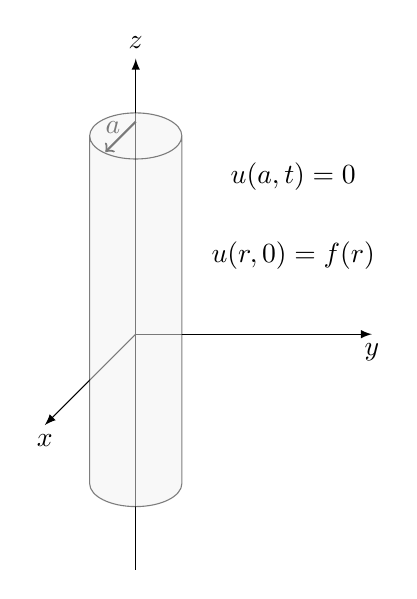
\begin{tikzpicture}

    \coordinate (O) at (0,0,0);
    \coordinate (A) at (3,0,0);
    \coordinate (B) at (0,3.5,0);
    \coordinate (C) at (0,0,3);
    \draw (0, 0, 0) -- (0, -3, 0);
    \draw [->, thick] (0, 2.7, 0) -- (0, 2.7, 1) node [above, pos=0.75] {$a$};
    % draw axis
    \draw[-latex] (O) -- (A) node[below] {$y$};
    \draw[-latex] (O) -- (B) node[above] {$z$};
    \draw[-latex] (O) -- (C) node[below] {$x$};

    \node[-latex] at (2, 2, 0) {$u(a, t) = 0$};
    \node[-latex] at (2, 1, 0) {$u(r, 0) = f(r)$};

    \node[cylinder, draw, shape aspect=.5, 
        cylinder uses custom fill, cylinder end fill=gray!10, 
        minimum height=1cm,
        cylinder body fill=gray!10, opacity=0.5, 
    scale=5, rotate=90]{};

    % \begin{scope}[shift={(4,0)}]

    % \coordinate (O) at (0,0,0);
    % \coordinate (A) at (2,0,0);
    % \coordinate (B) at (0,2,0);
    % \coordinate (C) at (0,0,3.5);

    %     % draw axis
    % \draw[-latex] (O) -- (A) node[below] {$y$};
    % \draw[-latex] (O) -- (B) node[above] {$z$};
    % \draw[-latex] (O) -- (C) node[below] {$x$};

    % \node[cylinder, draw, shape aspect=.5, 
    %     cylinder uses custom fill, cylinder end fill=green!50, 
    %     minimum height=1cm,
    %     cylinder body fill=green!25, opacity=0.5, 
    % scale=3, rotate=-135]{};
    % \end{scope}
    % \begin{scope}[shift={(8.,0)}]

    % \coordinate (O) at (0,0,0);
    % \coordinate (A) at (2,0,0);
    % \coordinate (B) at (0,2,0);
    % \coordinate (C) at (0,0,2);

    %     % draw axis
    % \draw[-latex] (O) -- (A) node[below] {$y$};
    % \draw[-latex] (O) -- (B) node[above] {$z$};
    % \draw[-latex] (O) -- (C) node[below] {$x$};


    % \node[cylinder, draw, shape aspect=.5,  
    %     cylinder uses custom fill, cylinder end fill=green!50, 
    %     minimum height=1cm,
    %     cylinder body fill=green!25, opacity=0.5, 
    % scale=3]{};


    % \end{scope}

\end{tikzpicture}
\end{document}